\section{Resultados} \label{sec:resultados}

	Nesta seção analisamos os resultados de nossa revisão sistemática. O propósito desta seção é dar uma visão geral de teste baseado em propriedades. Além disto, aproveitamos esta seção para responder as questões levantadas em nossa revisão sistemática.

	Para responder a primeira questão (\textit{Quais são os estudos atuais sobre "property-based testing "?}), são analisados os artigos que foram publicados entre 2017 e 2018. Dos trabalhos publicados em todo período de publicações $(2003-2018)$, cerca de $25,7\%$ foram publicados em 2017-2018, mostrando que este é um tema atual. Para uma melhor visualização do crescimento de publicações que envolvem testes baseados em propriedades, a Figura \ref{fig:crescimento}  mostra a evolução das publicações sobre do tema ao longo dos anos.

	\begin{figure}[!ht]
	  \centering
	  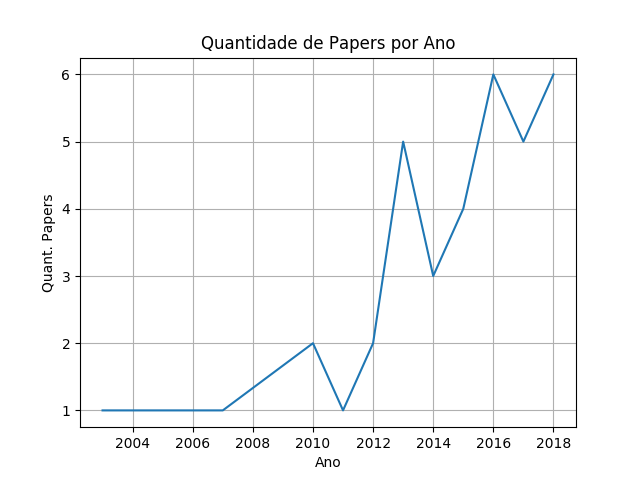
\includegraphics[scale=0.5]{Imagens/crescimento.png}
	  \caption{Crescimento do Teste Baseado em Propriedades ao longo dos anos}
      \label{fig:crescimento}
	\end{figure}

	Nos casos de estudo atuais do teste baseado em propriedades, há atualmente diferentes ramos de atuação dos artigos propostos. Grande parte dos artigos recentemente publicados utilizam o teste baseado em propriedades para aplicações,
	como \textit{web} \cite{peleg2018generating, martin2018property, chepurnoy2018checking, almendros2017web}  e \textit{block chain} \cite{aichernig2017property}. Enquanto alguns outros trabalhos \cite{loscher2018automating, hanus2016currycheck}, tem como objetivo o aperfeiçoamento deste tipo de teste. Em \cite{aichernig2017statistical} o teste baseado em propriedades é utilizado para simulação de modelos.


	%% qual vertente do property based testing está sendo mais usada -- considerando o tempo atual
	
	Sobre a segunda questão levantada (\textit{qual vertente do property based testing está sendo mais usada ?}), foi avaliado que grande maioria das aplicações de teste baseado em propriedades, considerando o tempo atual, são aplicações \textit{web}. Porém, além deste tipo de aplicações, existem abordagens em outros contextos como os já citados acima. Ao avaliarmos a quantidade de artigos publicados nos últimos anos (considerando período de $2017-2018$), cerca de $40\%$ são aplicações \textit{web}, o que nos auxiliou a chegar nesta conclusão. 

	%% quais são os pesquisadores mais influentes da área

	Para responder a quarta pergunta (\textit{quais são os pesquisadores mais influentes da área ?}) levantada na revisão sistemática, avaliamos os autores que mais publicam na área. Por meio da Figura \ref{fig:histograma} é perceptível que grande parte dos autores publicam apenas um artigo nesta área cerca de $72,2\%$. Enquanto outros autores, investem mais nessa área como por exemplo \textit{B. K. Aichernig e R. Schumi} os quais juntos possuem cerca de seis artigos na área, totalizando sozinhos $10\%$ dos artigos publicados no tema. Além desses, outros dois autores se destacam por ter dois artigos publicados na área, sendo eles: \textit{L. Fredlund et al} e \textit{K. Sagonas et al}.

	\begin{figure}[!ht]
	  \centering
	  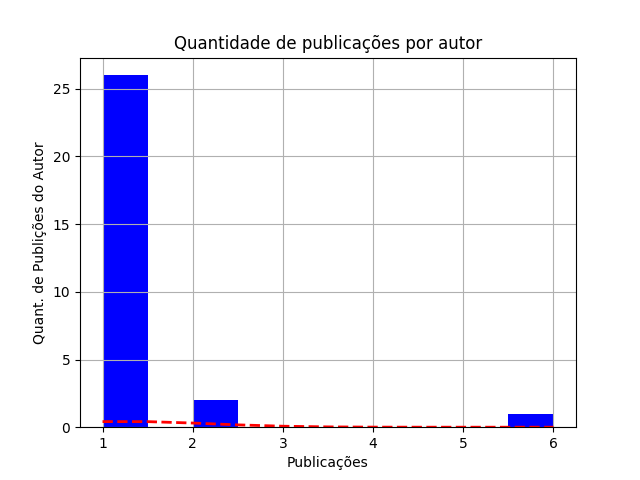
\includegraphics[scale=0.5]{Imagens/histograma.png}
	  \caption{Histograma que mostra a distribuição de artigos por autores}
      \label{fig:histograma}
	\end{figure}

	Avaliando quando estes artigos foram publicados, vemos que os autores \textit{B. K. Aichernig e R. Schumi} publicaram grande parte de seus artigos entre 2016-2018. Assim, concluímos que estes são os autores mais influentes nessa área em um período recente, dado o número de publicações e a abordagem das mesmas. Enquanto em um período menos recente, nos anos de 2014-2015 os autores que mais se destacam são \textit{L. Fredlund et al}.

	%% em qual domínimo está sendo aplicado

	Para avaliar os domínios em que a técnica de teste baseado em propriedades está sendo aplicada, foi realizada uma avaliação das palavras chaves presentes no artigo sendo estas sumarizadas por uma técnica de nuvem de palavras. Esta abordagem considera as palavras mais frequentes no texto para dar uma visão geral sobre as aplicações. Na Figura \ref{fig:cloud} é possível ver isto de maneira melhor.

	\begin{figure}[H]
	  \centering
	  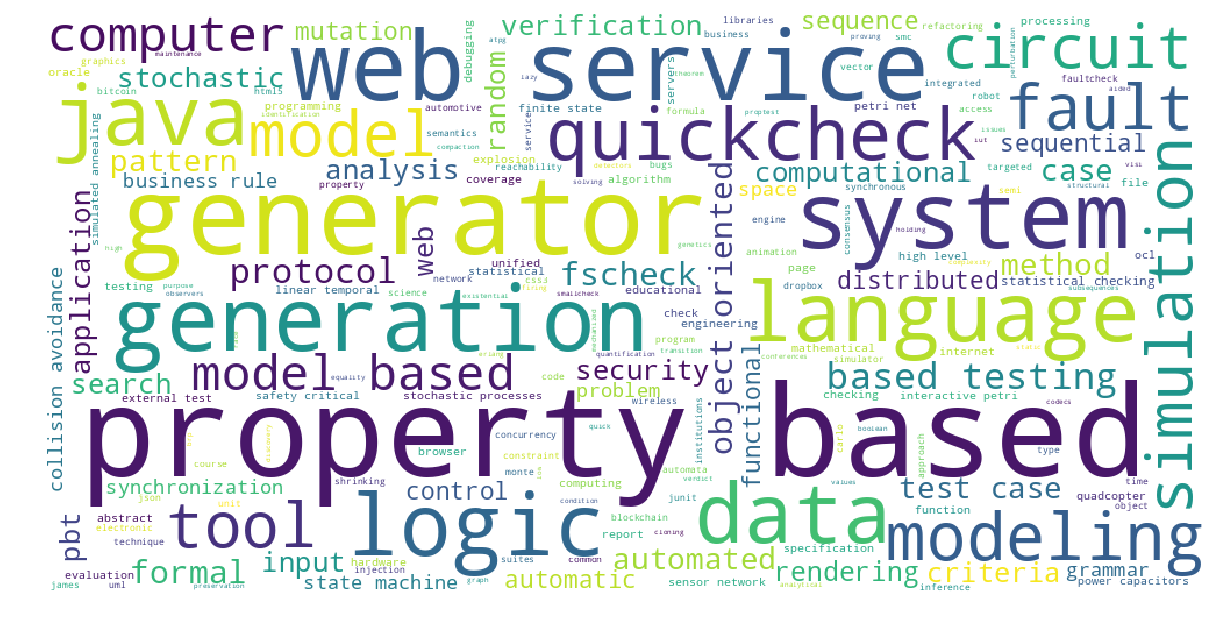
\includegraphics[scale=0.5]{Imagens/nuvem_palavras.png}
	  \caption{Nuvem de palavras}
      \label{fig:cloud}
	\end{figure}

	Por meio desta técnica de sumarização percebe-se que a abordagem é muito utilizada em linguagens \textit{web}, além de diversos paradigmas de programação como orientadas a objetos, funcionais e lógicas. Além destes, também é aplicada em domínios como segurança, \textit{block-chain} e mineração de dados (\textit{big data}), mostrando assim sua diversidade de aplicações e domínios, podendo esta ser aplicada em diversos contextos.